\section{Results}
\label{sec:results}

All experiments use Qwen3-32B and the v1 prompt (\S\ref{sec:model}; Appendix~\ref{sec:appendix_prompts}) unless noted; cross-model validation covers Dimensions~1--2, while secondary analyses (error taxonomy, DocRED $R^2$, Two One-Sided Tests [TOST]) remain single-model.

\begin{table}[t]
\centering
\small
\resizebox{\columnwidth}{!}{%
\begin{tabular}{llrrrrr}
\toprule
\textbf{Dataset} & \textbf{Embed.} & \textbf{$n$ pairs} & \textbf{$r$} & \textbf{$r^2$} & \textbf{95\% CI} & \textbf{$p$} \\
\midrule
Few-NERD & Qwen3 & 1{,}953 & 0.112 & 0.013 & {[}0.076, 0.156{]} & ${<}\,0.001$ \\
MAVEN & MiniLM & 11{,}026 & 0.129 & 0.017 & {[}0.104, 0.156{]} & ${<}\,0.001$ \\
\bottomrule
\end{tabular}}
\caption{Pairwise SCS--confusion correlation. Confusion rate is bidirectional $C(t_i{\to}t_j) + C(t_j{\to}t_i)$ divided by gold frequency sum; CIs are percentile bootstrap ($B{=}10{,}000$). FewRel ($r = 0.187$; \S\ref{sec:scs-validation}) excluded (per-instance RE format). Type-level cluster bootstrap CIs exclude zero (Few-NERD [0.069, 0.219]; MAVEN [0.081, 0.185]).}
\label{tab:pairwise}
\end{table}

\subsection{Count-Degradation Curves}
\label{sec:count_curves}

\looseness=-1
Figure~\ref{fig:main_results}a shows RE accuracy declines monotonically with schema size (85.7\%$\to$50.4\% for FewRel). NER recall drops from 0.72 (count 1) to 0.28 before recovering to 0.41 at full-schema. DocRED replicates the monotonic RE pattern (88.0\%$\to$38.7\%; Appendix~\ref{sec:appendix_figures}); MAVEN exhibits a reversed trend attributable to centrality confounding (\S\ref{sec:centrality_confound}). The decline is stable across seeds (Jonckheere-Terpstra $p < 0.001$) and replicates on Llama-8B ($-$43\,pp; Table~\ref{tab:cross_model}), Llama-70B, and Gemini Flash (Figure~\ref{fig:cross_model_count}).

\subsection{Pairwise Confusability and Type Confusion}
\label{sec:pairwise}

\looseness=-1
We test whether pairwise SCS predicts type-level confusion rates. For each type pair $(t_i, t_j)$, we compute the confusion rate (the fraction of $t_i$ gold instances misclassified as $t_j$) and correlate it with $\text{SCS}(t_i, t_j)$. Table~\ref{tab:pairwise} reports Pearson correlations with bootstrap 95\% confidence intervals (CIs).

\looseness=-1
The correlations are statistically significant but modest: $r^2 \approx 1.3\text{--}1.7\%$. Type-level cluster bootstrap yields wider but still significant CIs (Few-NERD: [0.069, 0.219]; MAVEN: [0.081, 0.185]; $B = 10{,}000$). Spearman correlations corroborate ($\rho = 0.144\text{--}0.227$; reaching $0.27\text{--}0.31$ among nonzero-confusion pairs).

\looseness=-1
While pairwise $r^2$ is modest, correlated type pairs within batches compound into substantial batch-level RE accuracy variance (\S\ref{sec:bcs_controlled}). Independent MiniLM embeddings yield stronger correlations ($r = 0.172$ vs.\ Qwen3 $r = 0.138$; Appendix~\ref{sec:appendix_bcs_sensitivity}); SCS outperforms simpler baselines (Appendix~\ref{app:scs-baselines}; concrete examples in Appendix~\ref{app:error-analysis}).

\begin{figure}[t]
\centering
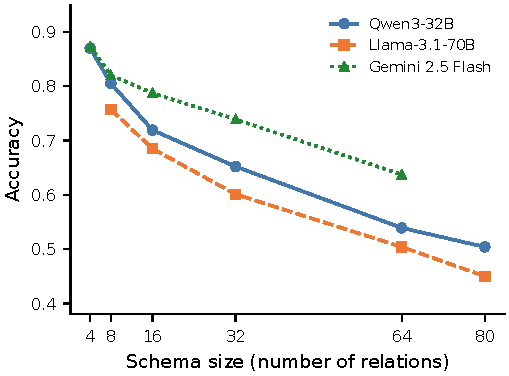
\includegraphics[width=\columnwidth]{../../figures/paper/fig_cross_model_count.pdf}
\caption{Cross-model count-curve replication on FewRel RE. All three model families show monotonic accuracy decline with schema size ($\rho = -1.0$ for Qwen3-32B and Gemini Flash on counts 4--32). Gemini shows shallower decline, consistent with ceiling compression.}
\label{fig:cross_model_count}
\end{figure}

\begin{figure*}[t]
\centering
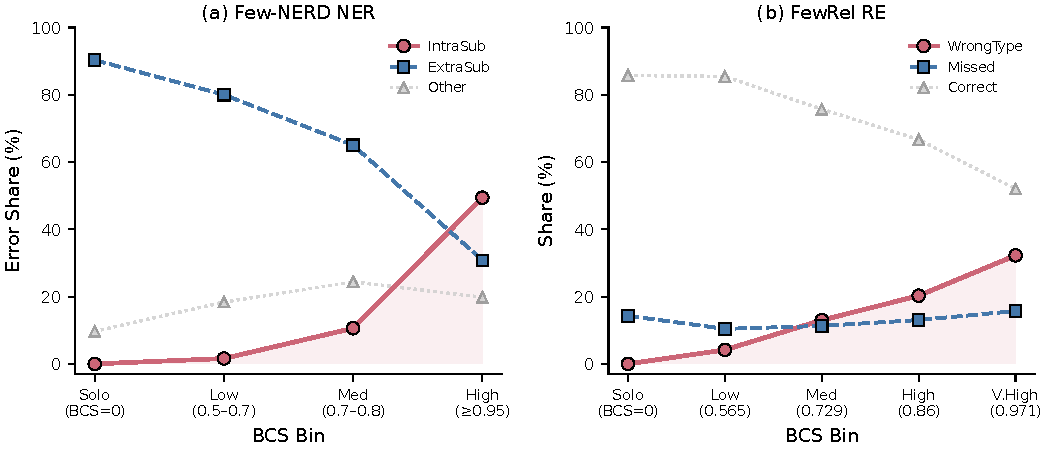
\includegraphics[width=\textwidth]{../../figures/paper/fig_error_taxonomy.pdf}
\caption{Error taxonomy decomposition (Few-NERD NER and FewRel RE). Intra-batch substitution (IntraSub) scales monotonically with BCS across all evaluated datasets ($\rho = 0.843\text{--}1.0$; Table~\ref{tab:error_taxonomy} includes DocRED). RE missed rates remain flat (10--16\%), but NER missed rates are substantially higher (43--65\%) and non-monotonic.}
\label{fig:error_taxonomy}
\end{figure*}

\subsection{BCS-Controlled Experiments}
\label{sec:bcs_controlled}

\looseness=-1
On FewRel, BCS independently explains ${\sim}$27\% of cross-batch RE accuracy variance (semipartial $R^2 = 0.273$, $n = 204$, after controlling for degree centrality), the primary quantitative evidence for confusability as a predictor alongside count. We fix type count and vary BCS to isolate this effect. FewRel's balanced design (700 instances per type) eliminates type frequency as a confound;\footnote{Partial correlation controlling for degree centrality: FewRel $r_{\text{partial}} = -0.537$ ($p < 0.001$, VIF${}\,=\,1.18$). DocRED partial correlation ($r_{\text{partial}} = -0.348$, $p < 0.001$) is reported for completeness, but VIF${}\,=\,50.9$ (BCS--centrality $r = 0.99$) renders the estimate unstable; the clean evidence for BCS's independent contribution comes from FewRel (Appendix~\ref{sec:appendix_partial_corr}, Table~\ref{tab:partial_corr}).} the within-pool analysis (\S\ref{sec:within_pool}) controls for pool composition. Adding domain entropy as a covariate leaves the BCS coefficient unchanged ($p_{\text{entropy}} = 0.97$; all VIF${}\,<\,2$; domain composition analysis in Appendix~\ref{sec:appendix_domain_distribution}).

In BCS-controlled FewRel subsets, extreme-batch construction yields $\Delta = -31.2$\,pp at 80 relations (95\% CI [17.7, 42.7]), stable across count levels (full data in Appendix~\ref{app:bcs-controlled-table}). An intermediate count${}\,=\,40$ evaluation confirms monotonic decline ($-$33.3\,pp at count 8, $-$31.8\,pp at count 16). DocRED extreme-BCS gaps persist ($-$25.0\,pp at count 16, $-$15.7\,pp at count 32; both $\rho < -0.69$) but semipartial $R^2_{\text{BCS}} = 0.056$ confirms 90\% of variance is shared with centrality (Appendix~\ref{sec:appendix_partial_corr}).

\paragraph{Within-pool and practical magnitude.}
\label{sec:within_pool}
\label{sec:practical_magnitude}
\looseness=-1
Within-pool analysis confirms slope consistency across pools (permutation $p \approx 0.60$; Appendix~\ref{app:within-pool-method}; CI interpretation in Appendix~\ref{sec:appendix_within_pool}). Cluster-robust inference confirms CIs are not inflated by shared instances (Appendix~\ref{sec:appendix_bootstrap_ci}). Amplification from pairwise $r^2 \approx 1.5\%$ to batch-level ${\sim}$27\% reflects correlated confusable-type interactions compounding within shared prompts \citep{robinson-1950-ecological,baan-2023-ecological} (${\sim}3\times$; Appendix~\ref{app:aggregation-sim}).

\paragraph{Cross-model validation.}
\looseness=-1
The count decline replicates across model families (Figure~\ref{fig:cross_model_count}). BCS effects also replicate: Llama-8B extreme-BCS gaps reach 77--87\% of Qwen3-32B's (Table~\ref{tab:cross_model_bcs}); Llama-70B confirms the effect at the 70B scale (Appendix~\ref{sec:appendix_cross_model_70b}); Gemini~2.5~Flash shows $\Delta = -17.6$\,pp (Appendix~\ref{sec:appendix_cross_model_gemini}). All three models show no NER BCS signal (Table~\ref{tab:cross_model_ner_null}), confirming task asymmetry.

\paragraph{Prompt sensitivity.}
\looseness=-1
The BCS gap remains significant under v2 prompt ($-$25.5\,pp, $r = -0.919$; Appendix~\ref{sec:appendix_prompt_sensitivity}) and across four structurally distinct prompt variants (all $r \leq -0.47$; Appendix~\ref{sec:appendix_prompt_variants}), ruling out prompt design as the source.

\subsection{Multi-Dimensional Degradation}
\label{sec:multi_channel}

\looseness=-1
Error taxonomy decomposition (Table~\ref{tab:error_taxonomy} and Figure~\ref{fig:error_taxonomy}) shows intra-batch substitution (IntraSub) scales monotonically with BCS across all three datasets ($\rho = 0.843\text{--}1.0$, all $p < 0.001$). In DocRED, IntraSub accounts for 72\% of errors in high-BCS batches vs.\ 15\% in low-BCS; extreme-BCS batches produce $9.9\text{--}27.5\times$ more confusion. Cross-model replication confirms the pattern on FewRel RE: Gemini~2.5~Flash ($\rho = 0.821$) and Llama-3.1-8B ($\rho = 0.430$; Table~\ref{tab:cross_model_error_taxonomy}).

\looseness=-1
These results establish two dimensions: \textbf{Dimension~1} (count predicts recall decline) and \textbf{Dimension~2} (confusability predicts type confusion). TOST \citep{lakens-2017-equivalence,schuirmann-1987-tost} bounds the FewRel interaction within $\pm 3$\,pp ($p = 0.003$; equivalence holds from $\pm 2$ through $\pm 5$\,pp; Appendix~\ref{sec:appendix_factorial}) In NER, batch-level BCS signal is not detected: errors distribute across miss, boundary, and type modes, and BCS range restriction limits power to 65\% (Appendix~\ref{sec:appendix_ner_power}); relaxed span matching does not recover a BCS signal either (Appendix~\ref{app:relaxed-matching}). Renaming and few-shot do not close the gap (Appendices~\ref{app:renaming},~\ref{sec:appendix_fewshot_bcs}).

\subsection{Centrality as a Potential Confound on Homogeneous Schemas}
\label{sec:centrality_confound}
\looseness=-1
Per-type analysis on MAVEN reveals an anomalous \emph{positive} BCS--F1 correlation ($\rho = +0.184\text{--}0.208$, $p < 0.03$): FrameNet-derived types cluster tightly \citep{cai-isotropy-clusters-2021}, conflating confusability with centrality. Controlling for log frequency and degree centrality, the correlation vanishes ($p > 0.2$; Appendix~\ref{sec:appendix_residualized_bcs}), though the pairwise SCS signal remains intact ($r = 0.129$, $p < 0.001$). Few-NERD's cross-domain schema shows the expected negative direction ($\rho = -0.293$, $p = 0.02$); mean BCS is reliable only for cross-domain schemas.

